\documentclass{scrartcl}

\usepackage{amssymb}
\usepackage{amsmath}
\usepackage{tikz}

%from a lecture by Badiou (November 18, 2006), Miguel Abreu Gallery, New York

\begin{document}
	
	\hspace{-3cm}
	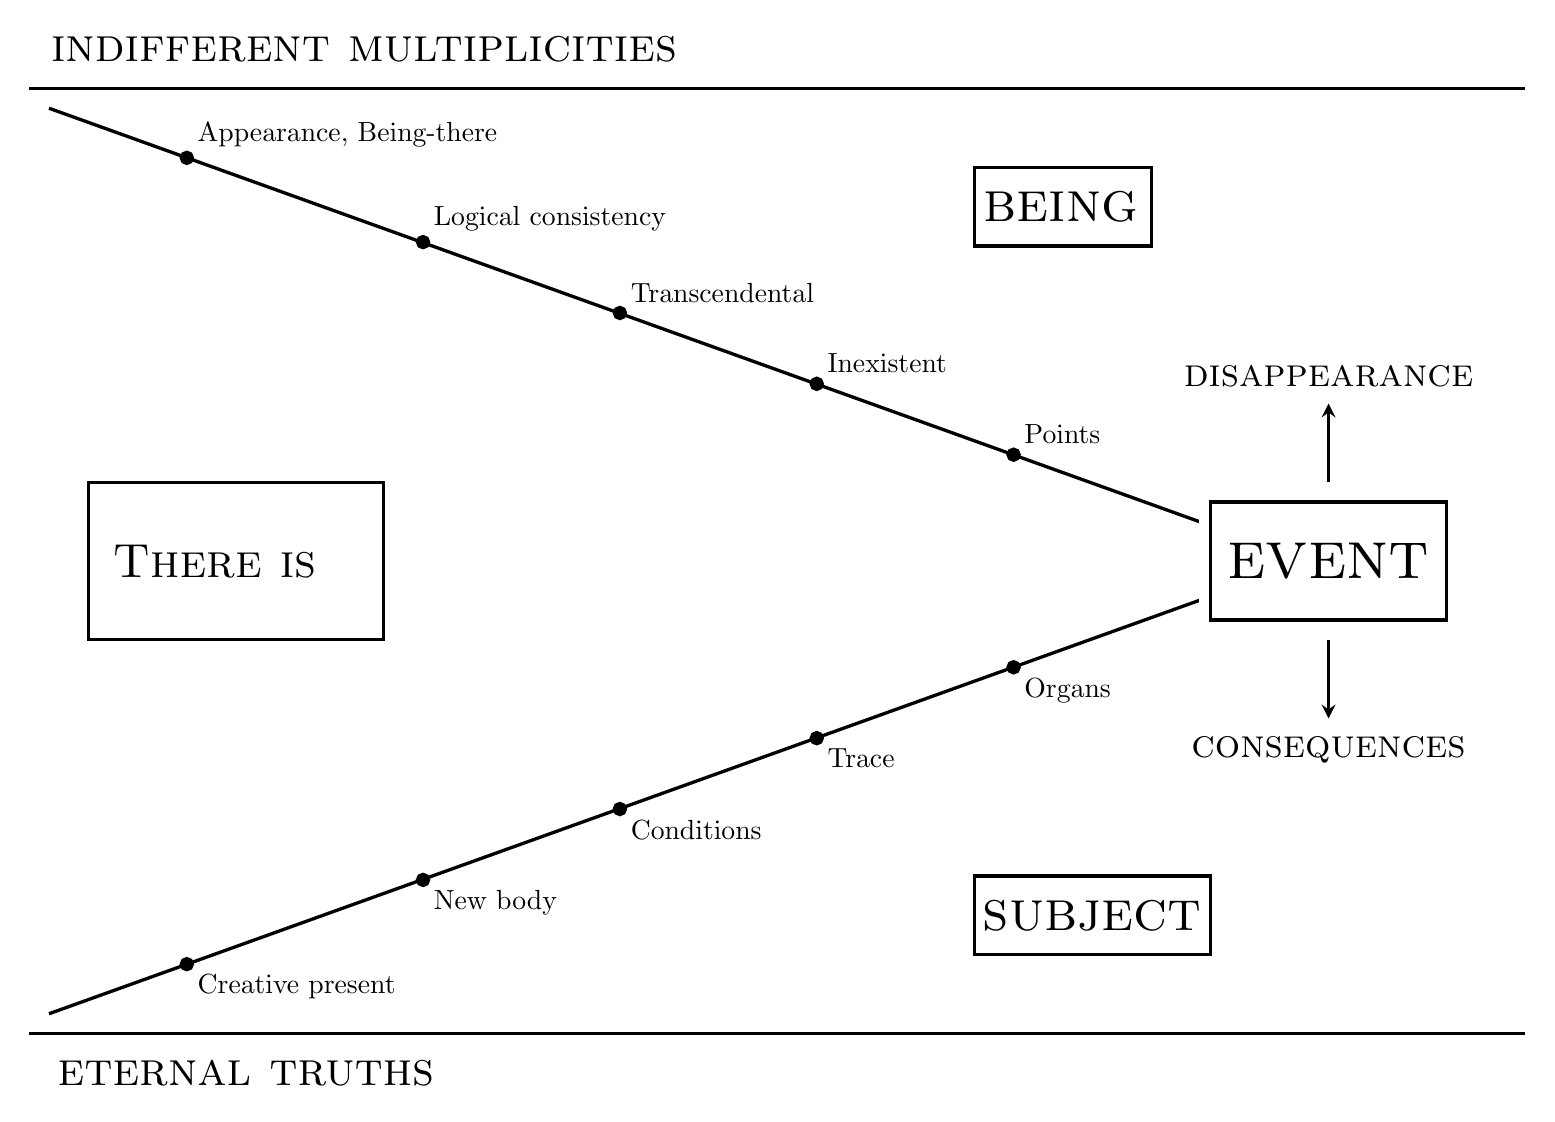
\begin{tikzpicture}[very thick]
	\draw (0,6)--(19,6);
	\draw (0,-6)--(19,-6);
	
	%diagonal lines
	\draw (0.25,5.75)--(16.25,0);
	\draw (0.25,-5.75)--(16.25,0);
	
	%boxes
	\fill[white] (14.85,0.75) rectangle (15,-0.75);
	\filldraw[draw=black,fill=white] (15,0.75) rectangle (18,-0.75);
	\node at (16.5,0) {\Huge \textsc{event}};
	\draw[->,>=stealth] (16.5,1)--(16.5,2);
	\node at (16.5,2.35) {\Large \textsc{disappearance}};
	\draw[->,>=stealth] (16.5,-1)--(16.5,-2);
	\node at (16.5,-2.4) {\Large \textsc{consequences}};
	%
	\filldraw[draw=black,fill=white] (0.75,1) rectangle (4.5,-1);
	\node at (2.35,0) {\LARGE \textsc{There is}};
	%
	\filldraw[draw=black,fill=white] (12,5) rectangle (14.25,4);
	\node at (13.1,4.5) {\huge \textsc{being}};
	%
	\filldraw[draw=black,fill=white] (12,-5) rectangle (15,-4);
	\node at (13.5,-4.5) {\huge \textsc{subject}};
	
	%dots
	\filldraw (2,5.12) circle (2pt) node[above right] {Appearance, Being-there};
	\filldraw (5,4.05) circle (2pt) node[above right] {Logical consistency};
	\filldraw (7.5,3.15) circle (2pt) node[above right] {Transcendental};
	\filldraw (10,2.25) circle (2pt) node[above right] {Inexistent};
	\filldraw (12.5,1.35) circle (2pt) node[above right] {Points};
	%
	\filldraw (2,-5.12) circle (2pt) node[below right] {Creative present};
	\filldraw (5,-4.05) circle (2pt) node[below right] {New body};
	\filldraw (7.5,-3.15) circle (2pt) node[below right] {Conditions};
	\filldraw (10,-2.25) circle (2pt) node[below right] {Trace};
	\filldraw (12.5,-1.35) circle (2pt) node[below right] {Organs};
	
	%labels
	\node at (4.25,6.5) {\LARGE \textsc{indifferent multiplicities}};
	\node at (2.75,-6.5) {\LARGE \textsc{eternal truths}};
	
	%\draw[help lines] (0,-6) grid (19,6);
	\end{tikzpicture}
	
\end{document}